\section{Languages}
The preceding section described a representation for programs which is suitable for any language. 

\begin{figure}
\todo{source text $\to$ parse tree $\to$ AST $\to$ ... $\to$ object code}
\caption{\label{fig-text} High-level structure of conventional language tool-chain.}
\end{figure}

In a conventional language, the structure of the language tool-chain imposes a one-way communication style (see Figure \ref{fig-text}). The programmer enters source text, using a text editor. This text drives the construction of the AST, and then the AST is transformed into object code. 

\temp{what's really happening: the programmer is using the text to manipulate the AST by indirect means}

\temp{limitations of text and parsing significantly constrain the communication}

\temp{feedback from compiler to programmer is constrained}

\temp{programmer mentally parses the code to understand the meaning}


\begin{figure}
\todo{source AST $\to$ kernel language $\to$ object code \emph{AND} $\to$ presentation language $\to$ visual representation}
\caption{\label{fig-tree} High-level structure of \Meta.}
\end{figure}

In \Meta, the programmer manipulates the AST, and the system derives both the object code and the visual representation of the code from the AST (see Figure \ref{fig-tree}). Because editing is performed at the level of the AST, there is no need for the programmer to make inferences about the meaning of the code.


\subsection{Grammars}
To define a particular language in this framework involves defining three aspects of the language.

The \emph{abstract syntax} of the language defines what nodes may appear in a program, and in what relationship to each other. In \Meta, abstract syntax is defined by a program in the \keyword{grammar} language. The grammar program acts as a specification which defines what programs are (syntactically) valid. 

Every language must have a \emph{semantics} that gives its programs meaning. While there are any number of ways to specify semantics, or indeed to make use of languages and programs with only ill-defined semantics, the approach pursued here is that of one or more kernel languages and syntax extension. The example of Lisp shows this to be a successful strategy, so the experimental question is how well it applies in this new setting. When a grammar defines a node type, it may also define the semantics of the construct by means of a reduction to a more primitive construct.

With abstract syntax and semantics taken care of, the both the Lisper and the Programming Language Theorist have all they need and will go happily on their ways. However, we would like to go further than that, so one more element is needed. \emph{Concrete syntax} is what the user reads and writes. The goal is to take advantage of the new approach to do things with concrete syntax that are impractical or impossible to do with textual source code. In \Meta, the concrete syntax of each type of node is given as a reduction to a presentation language.

Thus the grammar defines all three aspects of the language. The abstract syntax is defined \emph{prescriptively}, by determining what programs are legal. Both the semantics and concrete syntax are defined \emph{operationally}, as declarations of what reduced program and what visual representation will be derived from each source node.


\subsubsection{Abstract Syntax}
A program is \emph{valid} with respect to a \emph{grammar} if all of its node's types, values, and references comply with certain restrictions imposed by the grammar. For each node type, a grammar specifies:
\begin{enumerate}
\item Zero or more \emph{abstract types}, which are types for which the type being introduced is an \emph{instance}.
\item Whether the node's value should be an boolean, integer, string, sequence, or map.
\item For an integer-valued node, a range of legal values.
\item For a sequence node, the number and (abstract) type of expected child nodes.
\item For a map node, the expected attributes and the (abstract) types of nodes that may inhabit each of them.
\end{enumerate}

Because constraints on child nodes are declared via abstract types, the grammar is modular. A new instance of any node type can be introduced later without changing the definition of any node that might use it. It's like a very simple type system. 

\temp{When declaring a type to be an instance of an abstract type, one is bound to provide a compatible reduction, but there is no check that this is the case.}

\todo{need a different word than ``abstract''? Confusion with abstract syntax? non-terminal?}

A grammar may not specify every interesting property of a language. That is, not every syntactically valid program is correct. Depending on the nature of the language being defined, additional, more ambitious specifications can define additional properties (e.g. proper use of lexically-scoped variables or type safety). The abstract syntax is meant to be an easily-defined first step, and indeed in some sense it \emph{is} the language.

\subsubsection{Reductions}
A grammar may supply one or two reductions for each node type. These reductions are compiled into functions which are used in \todo{} (see section \ref{reduction}). Using a meta-programming approach, the reductions are economical and simple to define, but the full host language is available for use in reductions when needed.

An \keyword{expand} reduction is used to reduce a node in preparation for evaluation or execution, and therefore defines the semantics of the node. The result of this reduction is a node in the \emph{target language}. The declaration of a node type does not provide an \keyword{expand} reduction if the node's semantics is defined externally; in that case the un-reduced node is already in target-language syntax.

A \keyword{display} reduction reduces a node to a presentation language node. This reduction will always be present except in certain special cases which will be described later.

\begin{figure}[ht]
%  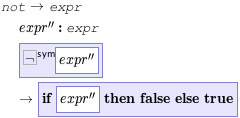
\includegraphics[scale=0.8]{src/image/not.png}  % 72dpi/0.8 = 90dpi for display

  \todo{re-capture with improved pres. for grammar}

  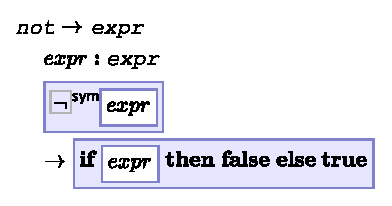
\includegraphics{src/image/not.pdf}

  \caption{\label{fig-and} Declaration of the \keyword{not} node for logical negation, taken from the \keyword{grammar} for the \Meta\ core language.}
\end{figure}

Figure \ref{fig-and} shows a simple declaration which includes all these elements. Because  the abstract syntax, semantics, and concrete syntax of every language construct are defined together in a simple, declarative style, each language construct is self-documenting. This flavor will be maintained in more interesting examples to come. By contrast, in a conventional language the concrete and abstract syntaxes are defined implicitly by the parser, and the semantics is defined somewhere inside the compiler. If there's any documentation, it has to be produced by a separate effort\footnote{If a \emph{parser generator} is used, then it may be able to produce some documentation of the syntax from the grammar. However in practice this kind of generated documentation tends to be difficult to use, due to the relative complexity of grammars that are meant to be used for parsing.}.


\subsubsection{Extending the Grammar Language}
Because a grammar is a \Meta\ program, the same tools for syntax extension are available for use in grammars, so the \keyword{grammar} language just described should be viewed as a starting point. It is meant to be general enough to define typical languages, and to handle most basic common needs for defining syntax. There are a couple of ways this language could be extended to provide additional power.

Using syntax extension, new kinds of node declarations could be supported. For example, an \keyword{infix} node declaration would require only an operator symbol and an expression to evaluate given two arguments. It would reduce to a declaration of a sequence node type,  requiring 2 or more argument expressions, a presentation reduction taking care of interposing the operator, and a left-to-right reduction of the arguments. \todo{actually, that would be awesome. should I implement it?}

Going further, a richer grammar language could provide additional specifications which would be consumed by a new checker. An example would typing rules. In this case, the enriched grammar would be reduced to the \keyword{grammar} language by discarding the extra information.


\subsection{Kernel Languages}
A \emph{kernel language} is one whose nodes have some fixed, pre-defined semantics (typically, they can be evaluated, yielding some specified result with some specified side effects). A complete language is built by \emph{extending} a kernel language with additional nodes whose semantics is defined in terms of reduction to (ultimately) the kernel language.

%\temp{This approach is exemplified by Scheme\cite{scheme}, in which only a handful of \emph{special forms} are pre-defined. All other language constructs are defined ``in the language'' in terms of macros which expand into the special forms. This works because Scheme (and Lisps in general) are meta-languages in the sense that programs are able to treat other programs as data. A macro definition takes the form of a function, called at compile time, which takes a piece of code as its argument and returns an expanded code fragment.}

One kernel language, the \emph{host kernel language}, is of particular interest, because it is the language the reductions themselves are written in. It is the glue that makes the system work. Requirements for the host kernel language:
\begin{enumerate}
\item Be in some sense minimal but sufficient that everything else can be done via extensions of it.
\item Be a meta-language, able to consume and produce nodes.
\item Fit well with the ``functional'' approach to nodes and trees.
\item Be easily implemented.
\end{enumerate}

In section \ref{host}, we'll describe the host kernel language of \Meta\ and how it fulfills these requirements.


\subsection{Presentation Languages}
The nodes of a \emph{presentation} language cast program elements in visual terms. A presentation language should be independent of the particular syntax of any one language, but might be suited to a particular family of related languages. More importantly, the presentation languauge should be flexible enough to represent any concievable construct that might be added to the source language. This is achieved by providing composable elements in the presentation language that can be combined in new ways to create new concrete syntax.

A presentation language is concrete in that it represents the program as it is presented to the user, however it is somewhat abstracted from the details of rendering characters and pixels. The reduction from source to presentation language is therefore quite direct and simple. Once the program is reduced to the presentation language, lower-level processing takes care of the details of rendering. This lower-level processing is common to all languages that reduce to the same presentation language, and does not need to be extended in the typical course of using (and extending) a source language.

\temp{different pres. languages for different domains - spreadsheet; word processor; flow-chart; ...}

\subsubsection{The \keyword{expr} Language}

\begin{figure}
\todo{capture from the implementation}
$$\keyword{keyword} = \mathit{str} : \keyword{string}$$
$$\keyword{int} = \mathit{str} : \keyword{string}$$
$$\dots$$
\caption{\label{fig-expr} Grammar for the \keyword{expr} language.}
\end{figure}

\Meta\ currently provides a single presentation language, \keyword{expr} (see Figure \ref{fig-expr}), which is well-suited to representing the expressions that make up the declarative portion of a typical modern programming language. However, it provides additional typographical sophistication, inspired by the familiar notation of algebraic expressions. An \keyword{expr} program is a tree made up of \emph{box} nodes. Each box node occupies a rectangular area of the rendering surface and always encloses the areas occupied by any child boxes. Several kinds of boxes are available in \keyword{expr}.

An \emph{atom} is a box that renders a sequence of characters and/or symbols using the normal spacing for text. Several types of atoms are available, each conveying what kind of entity the characters are meant to represent. When atoms are reduced to lower-level nodes, a distinctive typographical treatment is applied to each, as shown in Figure \ref{fig-atoms}. The list of atom types is meant to be expanded to serve the needs of any conceivable source language; the effort to add a new type is typically small (most simply specify a font and/or face), and in any case the total number of types in any one language is probably limited to a dozen or so, with much in common across languages, so we conjecture that the universe of useful atom types is not much larger than what \keyword{expr} currently provides. 

The diversity of atom types provides a measure of visual sophistication for programs, with a very small effort on the part of the language designer. Simply by identifying a visual style for each piece of syntax, some information about the meaning of each node is conveyed to the programmer. The particular treatment is meant to match the readability and high aesthetic standards of the pseudocode that might be found in a journal article or a good CS textbook.

\begin{figure}[ht]
\begin{tabular}{llll}
Type & Treatment & Examples & Typical use
\\
\hline
\keyword{keyword}
 & boldface
 & \keyword{true}
 & fixed language syntax
\\ & & \keyword{if} &   % Ugly hack! how to do proper multi-line cells in tabular env.?
\\
\hline
\keyword{var}
 & italic
 & $x$
 & names (user-provided or generated)
\\ & & $g$ & 
\\ & & $\mathit{fib}$ & 
\\
\hline
\keyword{num}
 & \textit{none}
 & 1
 & numerical literals
\\ & & 2.0 & 
\\ & & 3,000 & 
\\
\hline
\keyword{string}
 & sans serif
 & \textsf{abc} 
 & character literals (note special
\\
 & & \textsf{Hello,\textvisiblespace world} &  % open box: \u2423
  treatment of the space character)
\\
\hline
\keyword{name}
 & boldface, italic
 & \textbf{\emph{a}}
 & name literals
\\ & & \textbf{\emph{foo}} & 
\\
\hline
\keyword{mono}
 & monospaced
 & \texttt{nil}
 & external references
\\ & & \texttt{cons} & 
\\
\hline
\keyword{prod}
 & monospaced, italic
 & \texttt{\emph{expr}}
 & production names in grammars
\\ & & \texttt{\emph{left}} & 
\\
\hline
\keyword{symbol}
 & \textit{none}
 & $\to$
 & mathematical symbols
\\ & & $\in$ & 
\\ & & $\sum$ & 
\\
\hline
\end{tabular}
\caption{Types of atoms in \keyword{expr}, and the typographical treatment that is applied to them when \keyword{expr} is reduced. Note: the actual character content of each type of atom is arbitrary, except \keyword{symbol}, where the content must be one of a pre-defined set of available symbols.}
\label{fig-atoms}
\end{figure}

A similar idea leads to the \emph{syntax-coloring} behavior of many text editors, with a more cartoonish and less elegant result. \todo{figure comparing \Meta\ to Eclipse's editor with a similar expression, maybe? (see Figure \ref{fig-syntax-coloring}} In \Meta, using a single color for all syntax allows color differences to be used for other purposes.

\begin{figure}
\todo{get screenshots for something like this:}

\keyword{if} $(x < 5)$ \keyword{print}(``\textsf{foo}'');

\texttt{if (x < 5) print("foo");  // with crazy colors}

\label{fig-syntax-coloring}
\caption{Comparison of visual rendering of a simple Java expression, at 90 dpi. Note that most other figures that were captured from \Meta\ are rendered at full resolution, indicating the potential...}
\end{figure}

\emph{Composite} boxes contain child boxes which they arrange in a certain way. A \emph{sequence} is a horizontal arrangement of nodes separated by a certain amount of space. There are a handful of sequence types, each implying a certain amount of inter-node space. The amount of space is not just a visual thing; it indicates how tightly the sub-expression represented by the sequence binds, as we'll discuss in the next subsection. A \keyword{scripted} node contains a \emph{nucleus} and optional \keyword{sub}- and \keyword{super}(script) nodes. Special signs are similar to composites but also draw some particular glyph surrounding the child node(s). Examples are \keyword{radical} and \keyword{fraction}, used in very particular mathematical contexts.

A \keyword{delimited} node draws a pair of grouping symbols which expand to surround their contents. Available symbols include parentheses, various kinds of brackets, and the symbols for the $\lfloor\mathit{floor}\rfloor$, $\lceil\mathit{ceiling}\rceil$, and $|\mathit{magnitude}|$ operations.

An \keyword{embed} node signifies that its content represents code at a lower meta-level than the enclosing node (e.g. a quotation). An \keyword{unbed} node has the opposite effect. \temp{connection to upcoming subsection}

\temp{what am I doing with ``synthetic'' nodes? that is, nodes that are introduced during reduction, but do not represent actual source nodes? can any box be flagged?}

\keyword{expr} provides no real support for sequences of statements, or for larger constructs such as methods, classes and modules. These larger constructs pose additional problems for layout, such as how to handle indentation and whether lines should be wrapped and how, but the underlying concepts are similar. In \Meta, these larger groupings can be implemented somewhat awkwardly using the lower-level presentation language described later. 


\subsection{More Stuff}

\subsubsection{Parentheses}
Of particular interest is the handling of parentheses. At the AST level, it is never necessary for the programmer to use parentheses to make the meaning of an expression clear, because the intended order of operations is explicit in the structure of nodes. However, some indication of grouping may be needed at the presentation level to produce an unambiguous visual representation. In \Meta, these parentheses are introduced automatically after the program is reduced to the \keyword{expr} language. 

Thus the role of parentheses is turned around: instead of being provided by the programmer as a hint to the parser about how the expression should be constructed, they're provided by the system, as a form of feedback to the programmer about the structure of the program that's being written/read. \temp{...reflects the reality of the programmer/editor interaction, which is about iteratively making edits and then reading the resulting text -- it's not a question of coming up with the program in your head and then typing it out in a stream.}

The insertion of parentheses is handled in a language-independent way, taking advantage of the way expressions are represented in the \keyword{expr} language. Pairs of parentheses (in the form of a \keyword{delim} node) are inserted around a sequence if it is nested within another node in such a way that the resulting notation would otherwise be misleading. By taking over the notational details, \Meta\ relieves the programmer of a sometimes tedious task, but more importantly ensures that the visual form of the program always corresponds closely to the actual meaning.

For example, consider the following pair of related expressions:
$$n! - 1 \qquad \qquad \qquad \lsyn n - 1 \rsyn !$$
In the first expression, $n$ factorial is calculated first, and then 1 is subtracted from that. The tighter binding of the factorial operation is visually suggested by the juxtaposition of $n$ and $!$ with no space between. The second operation is displayed with thick spaces interposed, suggesting looser binding. Thus the visualization matches the expression's structure without any additional fuss. In contrast, in the second expression, the usually tighter-binding operation is performed second, so a pair of parentheses is inserted around $n-1$ to indicate the proper order. 

A handful of simple rules determine when parentheses are inserted, depending on the type of the parent and child node, and a few special cases (for example, a \keyword{nucleus} needs parens, but \keyword{super} and \keyword{sub} nodes do not). Figure \ref{fig-parens} shows several additional examples that cover most of the cases\footnote{Knuth in the TeXbook (p.\:140): ``\dots takes a bit of mathematical knowhow, since parentheses sometimes need to be inserted in order to preserve the meaning of the formula\dots If you are a typist without mathematical training, it's best to ask \dots for help.'' If Knuth had implemented this algorithm, his typists would have been spared this chore. However making the process manual does give the author a greater degree of control, which is probably appropriate in the context of publishing.}.


\begin{figure}[ht]
\todo{use my own output, which will be a better demonstration anyway}
$$
\begin{array}{ccc}
\lsyn 1+2 \rsyn \!\cdot\!3 & 
  \mathrm{\it vs.} & 
  1 + 2\!\cdot\!3
\\
\vspace{6pt}
\\
{\lsyn x+2 \rsyn}^i &
  \mathrm{\it vs.} & 
  x^{i+2}
\\
\vspace{6pt}
\\
{\lsyn a+b \rsyn}/2 & 
  \mathrm{\it vs.} & 
  {{a+b} \over 2}
\\
\vspace{6pt}
\\
{\lsyn y-1 \rsyn}^{1/2} + 2 & 
  \mathrm{\it vs.} & 
  \sqrt{y-1} + 2
\end{array}
$$
\caption{Examples of expressions that require parentheses (on the left), and related expressions where the notation is unambiguous and no parentheses are needed (on the right). Note that in cases where the meaning is equivalent, one or the other form might be preferable from an aesthetic point of view, but the transformation from one to the other is not necessarily trivial (see footnote). All examples are output from \Meta, with parentheses inserted automatically.}
\label{fig-parens}
\end{figure}

From the point of view of the language-definer, the impact is that there's no need to define or to document rules about operator precedence; you simply supply the desired notation. The \keyword{expr} language provides enough levels of spacing (four) to handle a moderately complex expression without parentheses. For example \todo{use actual output?}:
$$\keyword{if} \quad x \: < \: y + c! \quad \keyword{then} \quad \dots$$
Contrast this with textual languages: C has about 15 fixed precedence levels for its infix operators, C++ has 18, and Haskell allows new operators to be defined at any of 9 levels. This apparent bounty is misguided; it allows the programmer to avoid a little typing but is a ``notorious source of bugs''\cite{realworldhaskell} when the compiler and human reader don't agree on an expression's meaning.

% ``Even more importantly, complex expressions that rely completely on operator precedence are notorious sources of bugs. A compiler and a human can easily end up with different notions of what even a short, parenthesis-free expression is supposed to do.
%``There is no need to remember all of the precedence and associativity rules numbers: it is simpler to add parentheses if you are unsure.'' - Real World Haskell



\subsubsection{Embedding (Quotations) [todo]}

\temp{how embedding makes meta-programs comprehensible}

\temp{dual interpretation: code vs. visual template}

\temp{example of a presentation reduction with a conditional first? n-ary AND?}


\subsubsection{Names [todo]}
Another element of programs that gets special treatment 



\subsection{ASTs at Runtime}\todo{}

\temp{how much is there to say here? leave it to example 3?}


\temp{random comment: Note that grammars are currently defined as discrete programs, but in a real language the grammar might be constructed as the program is loaded and syntax declarations are processed.}



